% !TEX root = paper.tex
% !TEX encoding = UTF-8 Unicode
% -*- coding: UTF-8; -*-
% vim: set fenc=utf-8
% !TEX spellcheck = en-US
\section{Results}
\label{sec:results}



%------------------------------%
%: see Figure~\ref{fig:results}
\begin{figure}%[!ht]%%[p!]
\centering{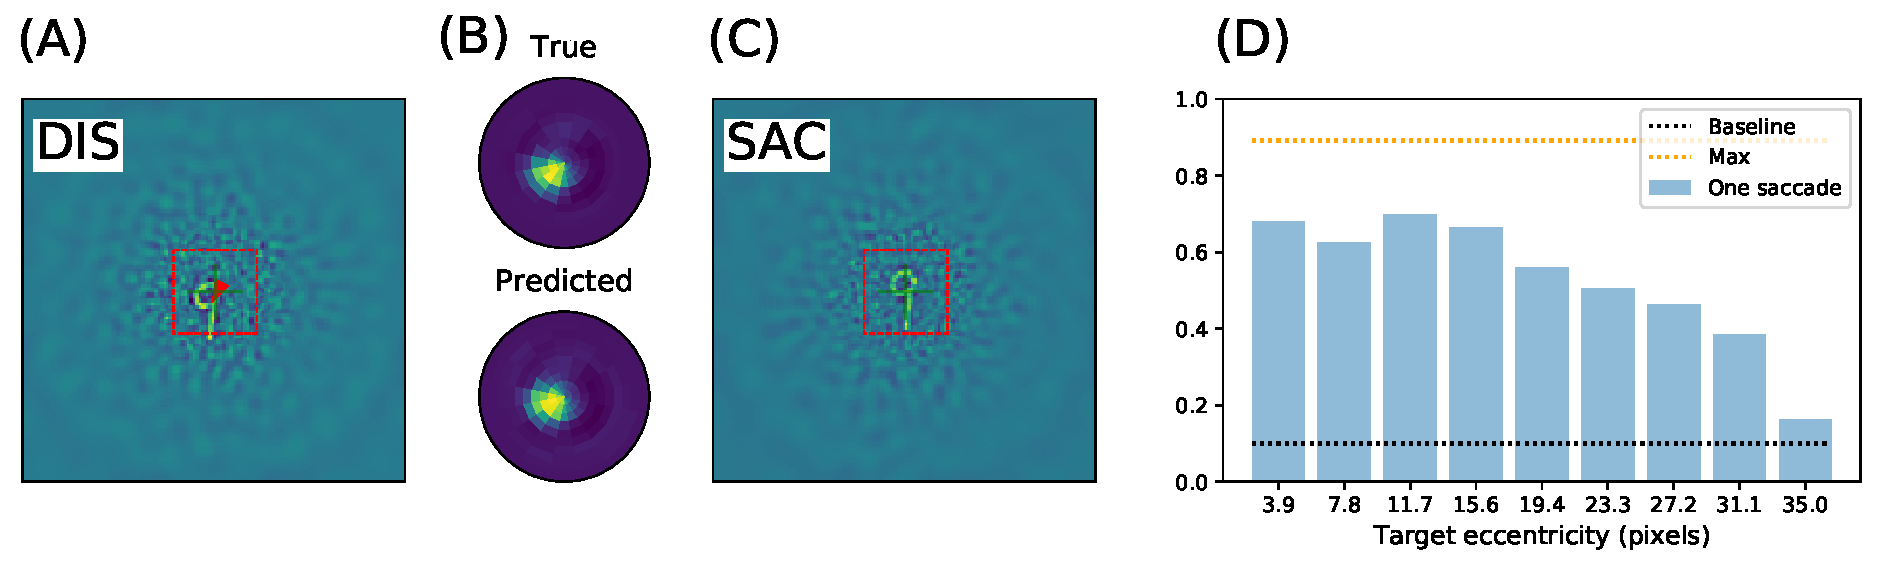
\includegraphics[width=\linewidth]{fig_result}}
\caption{
{\bf Results}: Results from simulations of the active vision agent.
(A)~The input image ('DIS', see  Figure~\ref{fig:results}-C)  is transformed ointo a retinoptopic representation which is used as the input to the 'Where' pathway of the agent. This pathway is a function that transforms this retinal image into a map predicting (B)~the accuracy of a classification in the 'What' pathway. The network fitting for this functiopn is trained in a supervised using a ground truth ('True') and we show here a prototypical example of the 'Predicted' map. This allows to (C)~generate a saccade to the most likely position in visual space to achieve a succesful classification. (D)~Testing over a range of $XXX$ different trials (different positions and digits), we show here the final average classification accuracy as a function of eccentricity. This shows first the results of the 'What' pathway ('No saccade') which quickly drops to baseline level after 3 scales. Second, we show the accuracy results obtained after one saccade which now drops to 'baseline' after 7 scales. This shows that by performing only one saccade, the image is now partly covered.
\label{fig:results}}%
\end{figure}%
%%------------------------------%
%result


% energy consumption


% inhibition of return
A particular property of our agent
is that at the time when the initial
input is presented, two independent inferences
are implemented. First, a classification
is performed by the 'what' pathway which
gives potentially the identity of the digit.
Second, an accuracy map is predicted
by the 'Whene' pathway. A possible heuristic
is therefore to compare the two maps to
chose the most appropriate action: either
the accuracy is best in the 'what'
patharay and in that case no saccade
is produced. In the other case, a
saccade is produced. In that case and
knowing the accuracy predicted by the
what pathway, one can update the
accuracy map of the 'where' pathway.
Indeed, one knows in particular the
accuracy of the 'what' pathway when
imposing small shifts to the input.
This allows in particular to Explain
away" the current ( 'fix') position and
those which are neighboring,(see figure
{fig: results} -No saccade). Such heuristic
gives a principled formulation of the
inhibition of return mechanism which
is an important aspect for modeling saccades.
In particular, we predict that such a
mechanism is dependent on the class
of inputs, and woulds -be different for
searching for faces as compared to digits.
